\documentclass[final]{beamer}

% ============================================================
% POSTER SETUP
% ============================================================

\usepackage[size=a0,orientation=landscape,scale=1.05]{beamerposter}

\usetheme{Madrid}
\usecolortheme{seahorse}

\setbeamertemplate{navigation symbols}{}
\setbeamertemplate{caption}[numbered]

\usepackage[utf8]{inputenc}
\usepackage[T1]{fontenc}
\usepackage[english]{babel}

\usepackage{amsmath,amssymb,mathtools}
\usepackage{bm}
\usepackage{booktabs}
\usepackage{array}
\usepackage{graphicx}
\usepackage{xcolor}
\usepackage{tikz}
\usetikzlibrary{positioning,arrows.meta}

% ============================================================
% COLORS
% ============================================================

\definecolor{posterblue}{RGB}{38,67,125}
\definecolor{posterlight}{RGB}{235,240,250}
\definecolor{posteraccent}{RGB}{40,125,130}

\setbeamercolor{block title}{
    fg=white,
    bg=posterblue
}

\setbeamercolor{block body}{
    fg=black,
    bg=posterlight
}

\setbeamercolor{headline}{
    fg=white,
    bg=posterblue
}

\setbeamercolor{footline}{
    fg=white,
    bg=posterblue
}

% ============================================================
% SOME MACROS
% ============================================================

\newcommand{\sigmoid}{\sigma}
\newcommand{\E}{\mathbb{E}}
\newcommand{\R}{\mathbb{R}}

% ============================================================
% TITLE
% ============================================================

\title{
Bayesian Inference for Spatial Poisson Models
}

\subtitle{
Exact posterior sampling by data augmentation and application to earthquake catalogues
}

\author{
 \textit{[authors]}
}

\institute{
\textit{[Affiliation]}
}

% ============================================================
% HEADER
% ============================================================

\setbeamertemplate{headline}{
    \begin{beamercolorbox}[wd=\paperwidth,ht=8cm,dp=1.5cm]{headline}
        \centering

        \vspace{0.8cm}

        {\fontsize{54}{60}\selectfont\bfseries
        \inserttitle
        \par}

        \vspace{0.35cm}

        {\fontsize{30}{34}\selectfont
        \insertsubtitle
        \par}

        \vspace{0.45cm}

        {\fontsize{25}{29}\selectfont
        \insertauthor
        \qquad
        \insertinstitute
        }
    \end{beamercolorbox}
}

% ============================================================
% FOOTER
% ============================================================

\setbeamertemplate{footline}{
    \begin{beamercolorbox}[wd=\paperwidth,ht=1.5cm,dp=0.7cm]{footline}
        \centering
        \large
        Spatial Poisson model --- preliminary results / work in progress
    \end{beamercolorbox}
}

% ============================================================
% DOCUMENT
% ============================================================

\begin{document}

\begin{frame}[t]

\vspace{0.2cm}

\begin{columns}[t,totalwidth=\textwidth]

% ============================================================
% ============================================================
% COLUMN 1
% MODEL + SAMPLER + ERGODICITY
% ============================================================
% ============================================================

\begin{column}{0.32\textwidth}

% ------------------------------------------------------------
\begin{block}{Spatial Poisson model}

We model the number of events in spatial cell $i$ as

\[
n_i \mid f_i
\sim
\operatorname{Poisson}(\lambda_i),
\]

with

\[
\lambda_i
=
\lambda \sigmoid(f_i),
\qquad
\sigmoid(f)
=
\frac{1}{1+e^{-f}}.
\]

The latent spatial field is assigned a Gaussian prior,

\[
f \sim
\mathcal N(\mu,Q^{-1}),
\]

where the precision matrix $Q$ introduces spatial dependence.

\vspace{0.3cm}

The posterior is

\[
p(f\mid n)
\propto
p(n\mid f)p(f),
\]

but it is \textbf{not Gaussian} because of the nonlinear
Poisson--sigmoid likelihood.

\end{block}


% ------------------------------------------------------------
\begin{block}{Data augmentation}

Instead of sampling directly from the non-Gaussian posterior,
we introduce two sets of auxiliary variables.

\vspace{0.5cm}

\begin{center}

\begin{tikzpicture}[
    box/.style={
        draw=posterblue,
        very thick,
        rounded corners,
        minimum width=5.1cm,
        minimum height=2.3cm,
        align=center,
        fill=white
    },
    >=Stealth
]

\node[box] (f) {
    Current field\\[2mm]
    $f^{(t)}$
};

\node[box, right=1.0cm of f] (k) {
    Auxiliary counts\\[2mm]
    $k$
};

\node[box, right=1.0cm of k] (w) {
    Pólya--Gamma\\[2mm]
    $\omega$
};

\node[box, right=1.0cm of w] (fn) {
    New field\\[2mm]
    $f^{(t+1)}$
};

\draw[->,very thick] (f) -- (k);
\draw[->,very thick] (k) -- (w);
\draw[->,very thick] (w) -- (fn);

\end{tikzpicture}

\end{center}

\vspace{0.5cm}

The auxiliary counts are

\[
k_i
\sim
\operatorname{Poisson}
\left(
\lambda\sigmoid(-f_i)
\right).
\]

Since

\[
\sigmoid(f_i)+\sigmoid(-f_i)=1,
\]

the augmented total

\[
b_i=n_i+k_i
\]

induces a logistic/binomial representation.

We then draw

\[
\omega_i
\sim
\operatorname{PG}(n_i+k_i,f_i).
\]

\end{block}


% ------------------------------------------------------------
\begin{block}{Gaussian conditional update}

After augmentation,

\[
f\mid n,k,\omega
\sim
\mathcal N
\left(
m_{\mathrm{post}},
Q_{\mathrm{post}}^{-1}
\right).
\]

The conditional precision is

\[
Q_{\mathrm{post}}
=
Q+\Omega,
\qquad
\Omega
=
\operatorname{diag}
(\omega_1,\ldots,\omega_N),
\]

and

\[
m_{\mathrm{post}}
=
Q_{\mathrm{post}}^{-1}
\left(
Q\mu+\kappa
\right),
\]

where

\[
\kappa_i
=
\frac{n_i-k_i}{2}.
\]


\end{block}




% ------------------------------------------------------------
\begin{block}{Computational structure}

For a spatial grid, the prior precision $Q$ is sparse.

Since the augmentation only adds the diagonal matrix $\Omega$,

\[
Q_{\mathrm{post}}
=
Q+\Omega
\]

remains sparse.

Thus the Gaussian update can exploit sparse Cholesky
factorization rather than dense covariance matrices.

\end{block}

\end{column}


% ============================================================
% ============================================================
% COLUMN 2
% SYNTHETIC EXPERIMENTS
% ============================================================
% ============================================================

\begin{column}{0.32\textwidth}


% ------------------------------------------------------------
\begin{block}{Experiment 1: elongated bars}

\begin{minipage}[t]{0.48\linewidth}
\centering

\textbf{True rate}

\vspace{0.2cm}

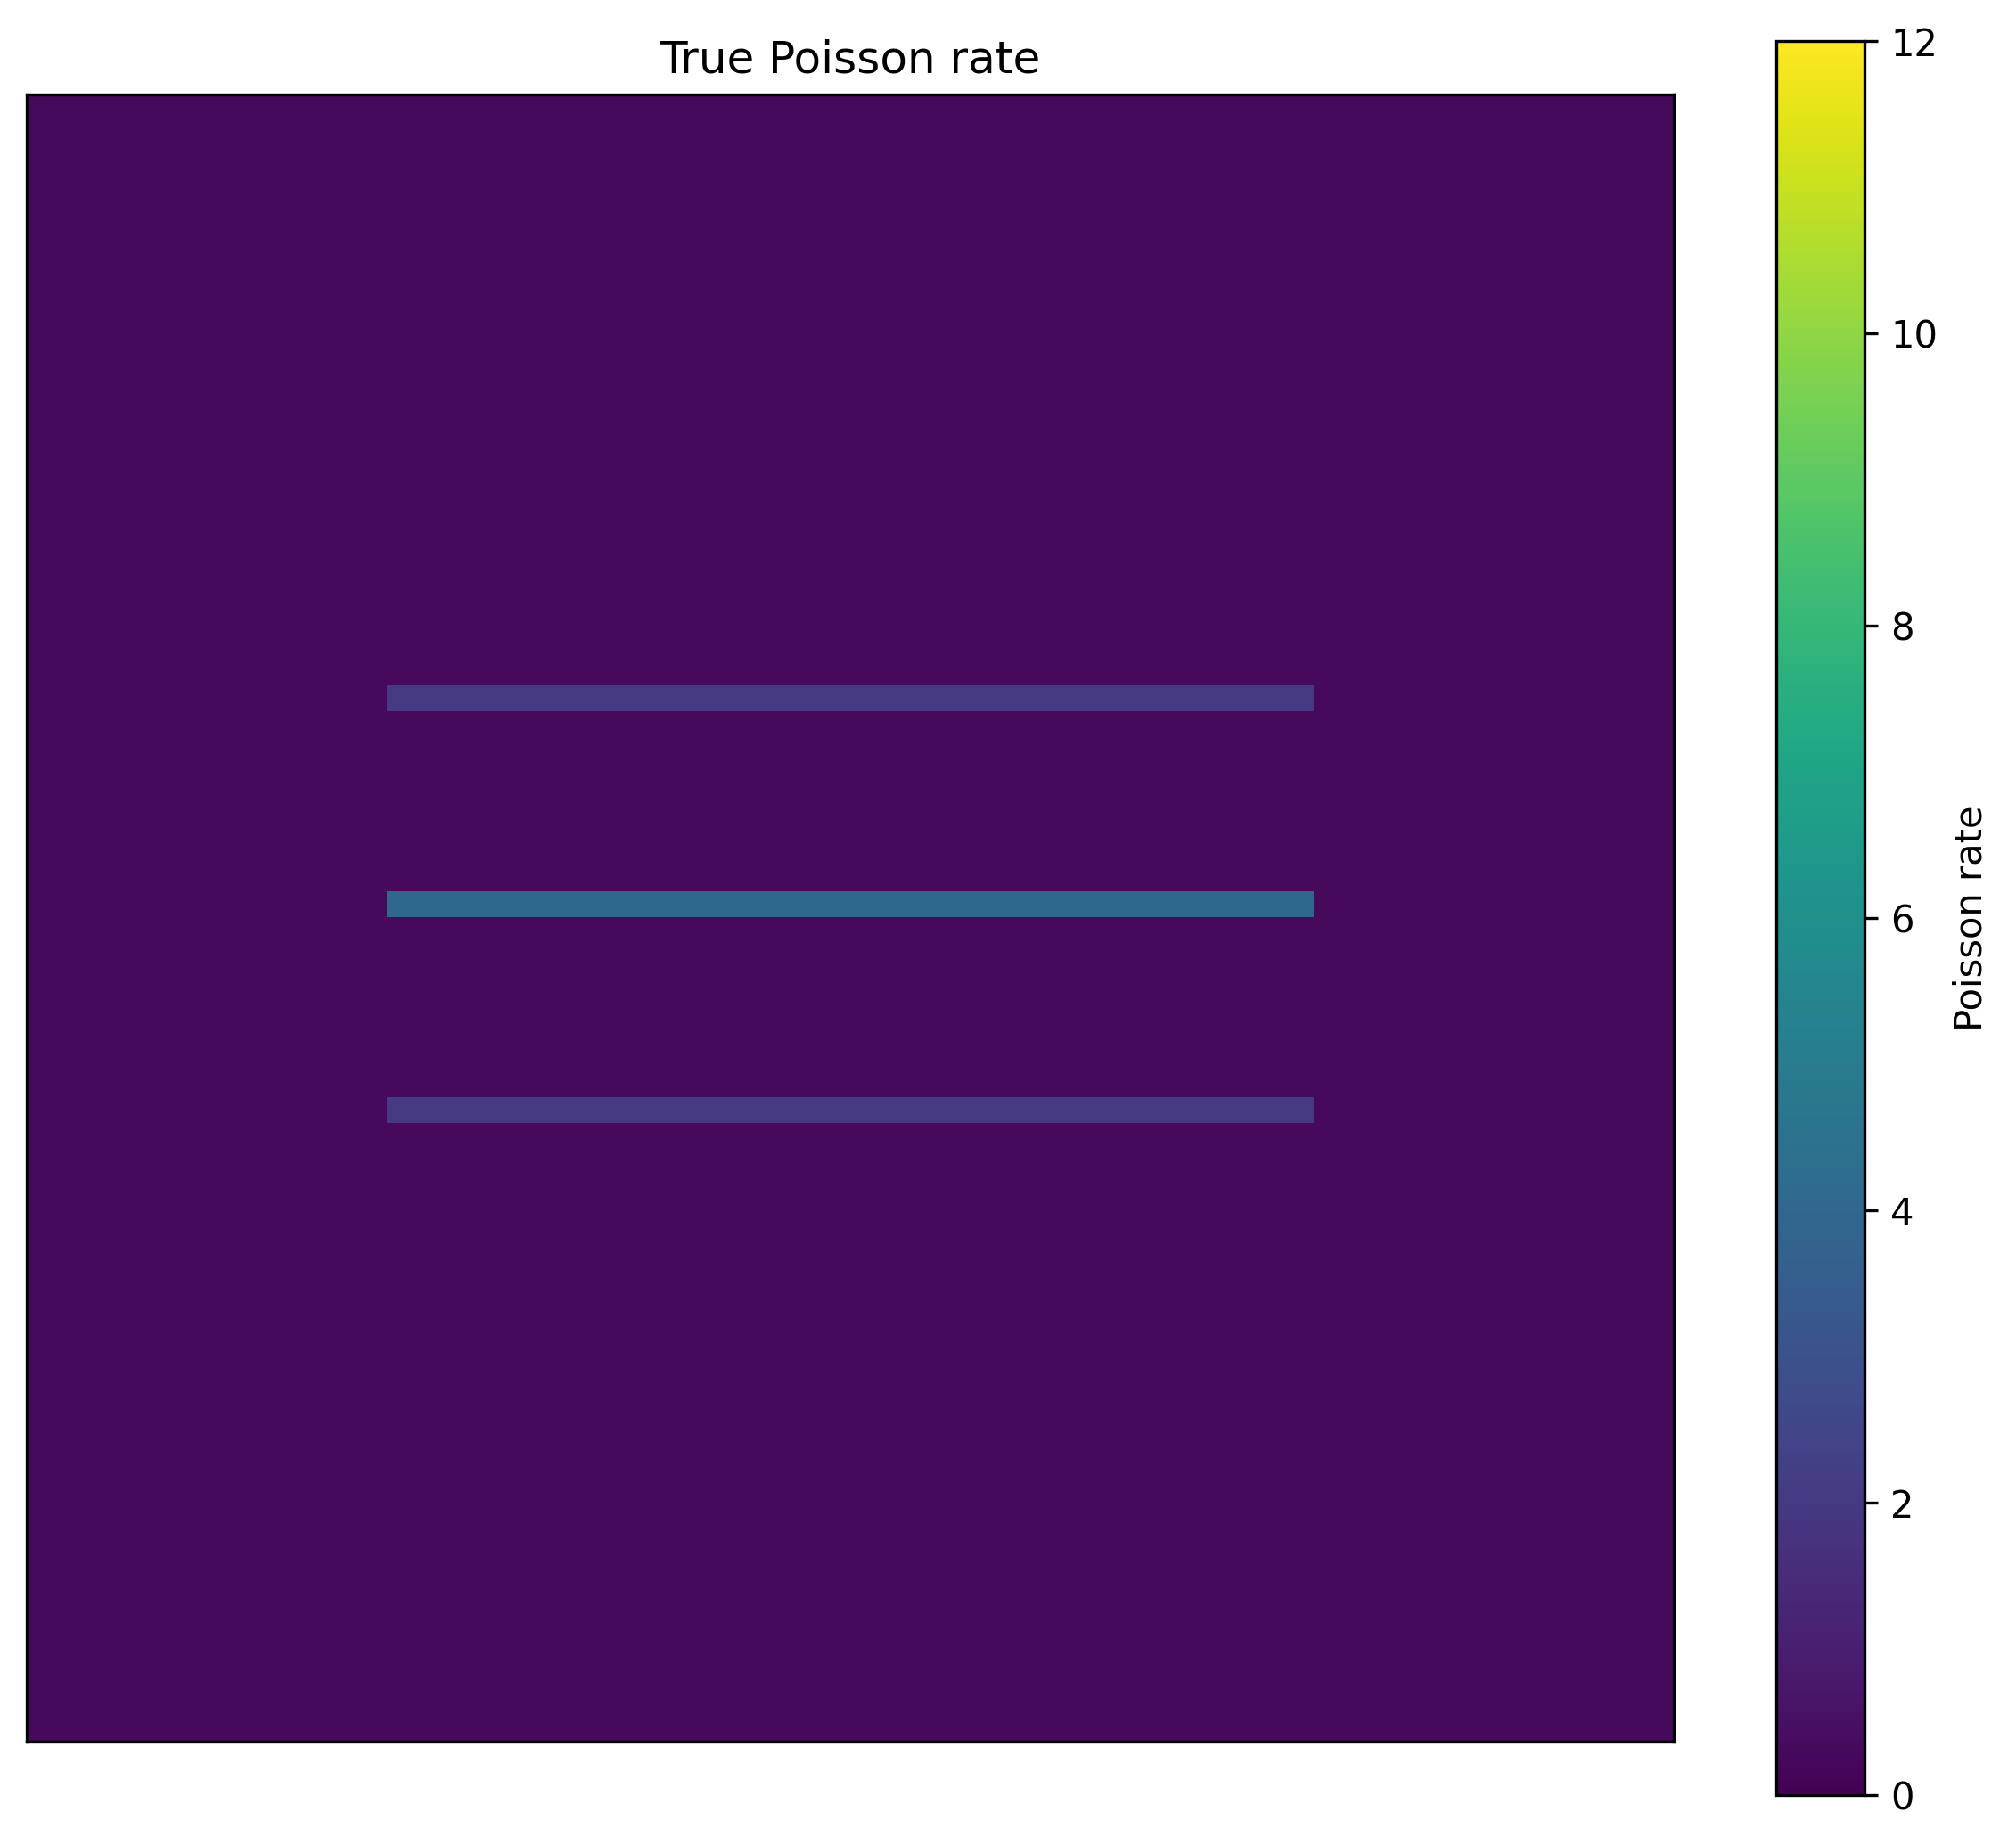
\includegraphics[
    width=\linewidth,
    height=13cm,
    keepaspectratio
]{figures/synthetic_bars_true_rate_rho_3_lam_12_var_4.png}

\end{minipage}
\hfill
\begin{minipage}[t]{0.48\linewidth}
\centering

\textbf{Observed counts}

\vspace{0.2cm}

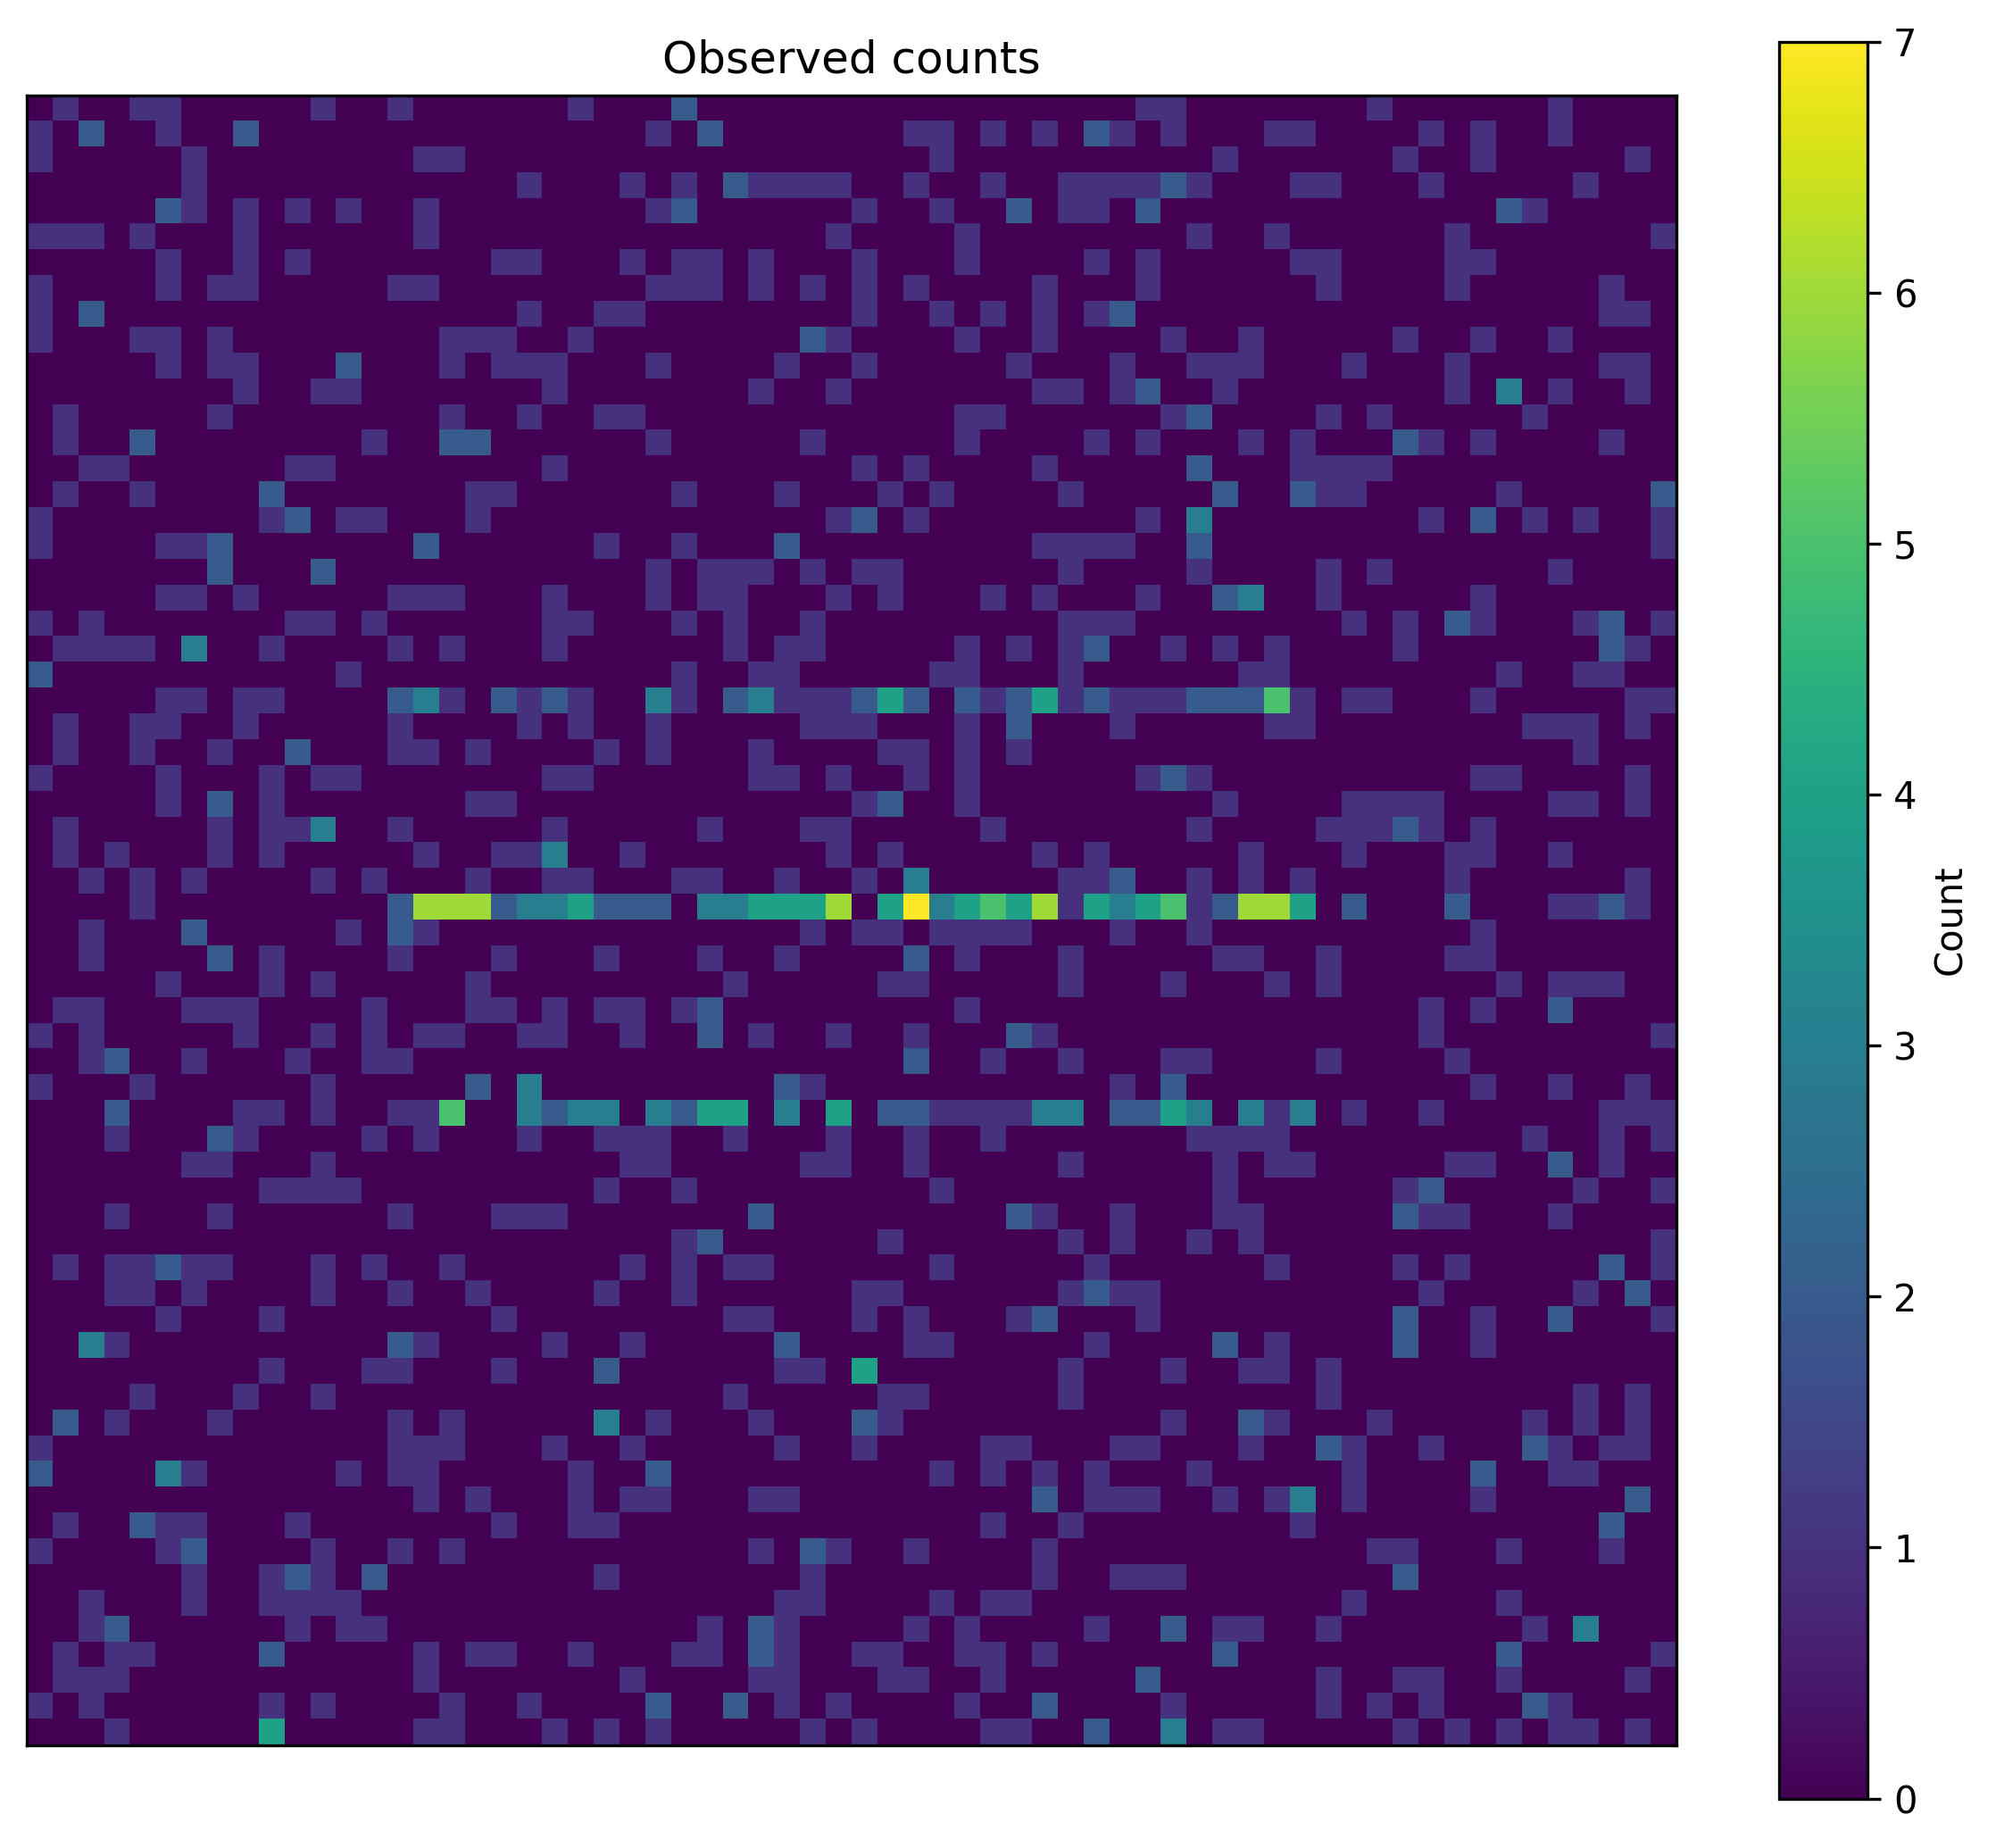
\includegraphics[
    width=\linewidth,
    height=13cm,
    keepaspectratio
]{figures/synthetic_bars_observed_counts_rho_3_lam_12_var_4.png}

\end{minipage}

\vspace{0.5cm}

\begin{minipage}[t]{0.48\linewidth}
\centering

\textbf{Posterior mean}

\vspace{0.2cm}

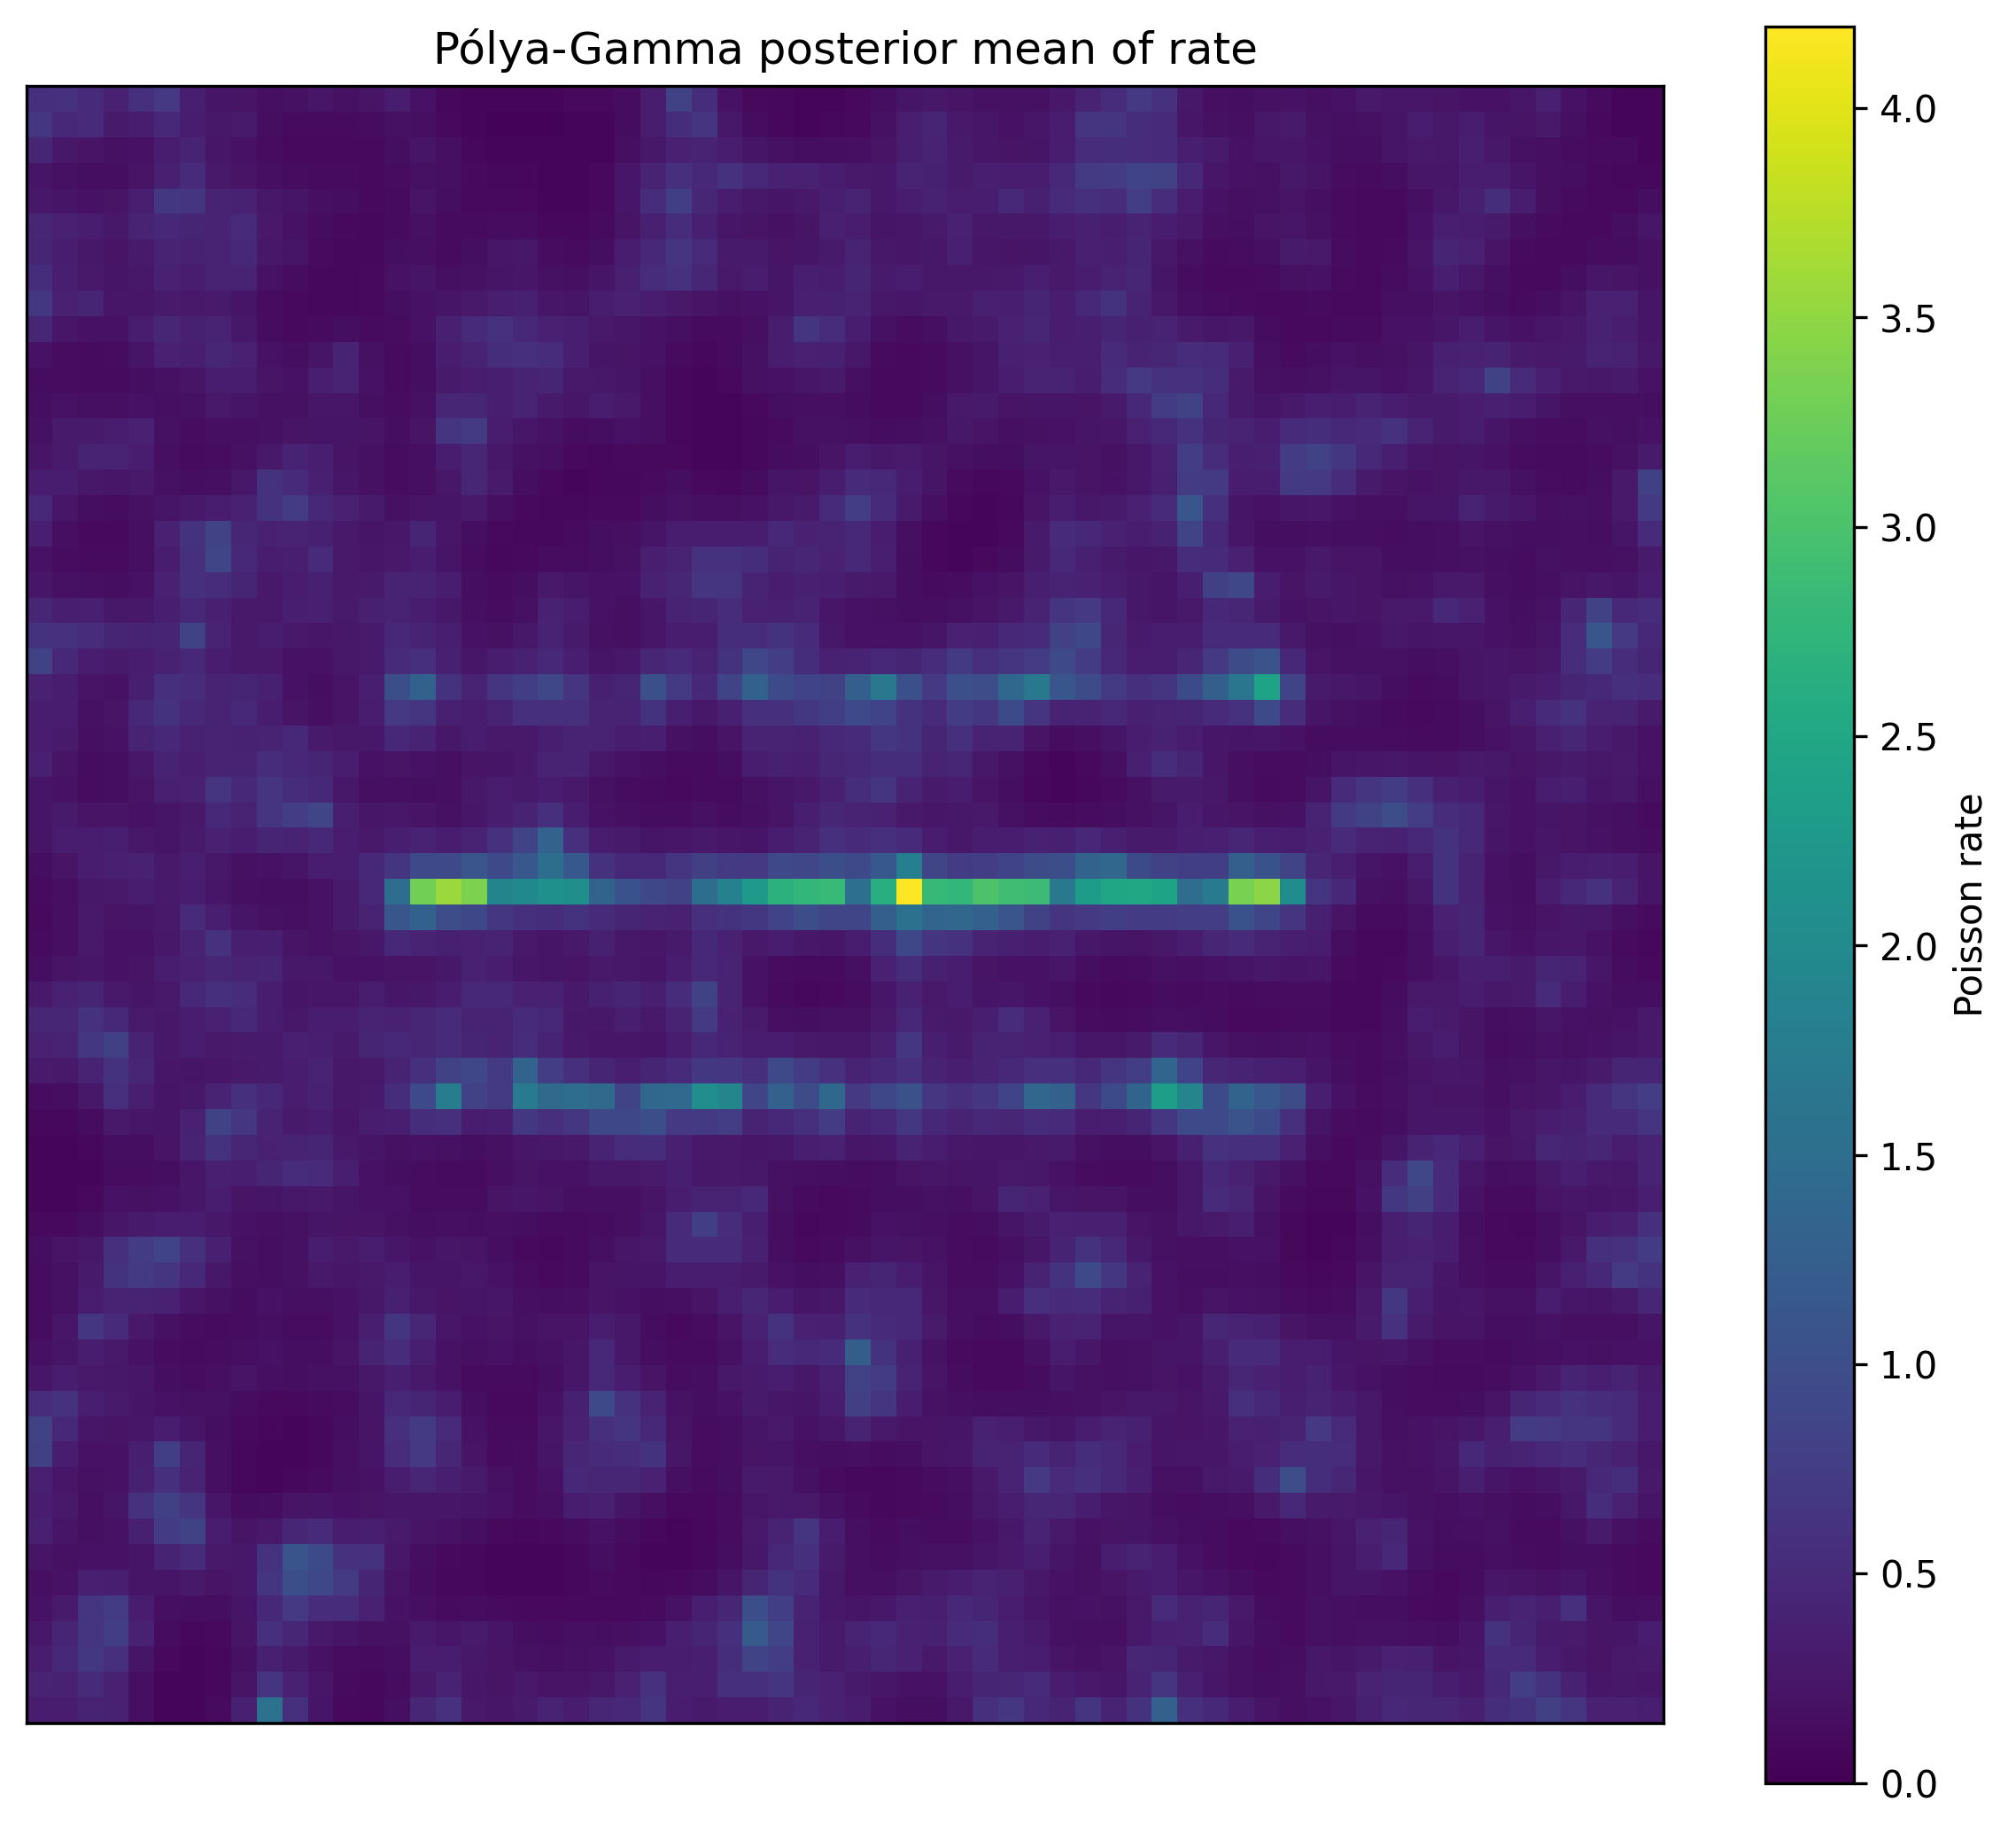
\includegraphics[
    width=\linewidth,
    height=13cm,
    keepaspectratio
]{figures/synthetic_bars_posterior_mean_rate_rho_3_lam_12_var_4.png}

\end{minipage}
\hfill
\begin{minipage}[t]{0.48\linewidth}
\centering

\textbf{Posterior mean $-$ truth}

\vspace{0.2cm}

\includegraphics[
    width=\linewidth,
    height=13cm,
    keepaspectratio
]{figures/synthetic_bars_posterior_mean_minus_truth_rho_3_lam_12_var_4.png}

\end{minipage}

\vspace{0.4cm}

\textbf{Result.}
The sampler identifies the elongated high-rate structures despite
strong Poisson noise. The largest errors occur close to the sharp,
narrow structures where the spatial prior induces smoothing.

\end{block}

% ------------------------------------------------------------
\begin{block}{Experiment 2: compact block}

\begin{minipage}[t]{0.48\linewidth}
\centering

\textbf{True rate}

\vspace{0.2cm}

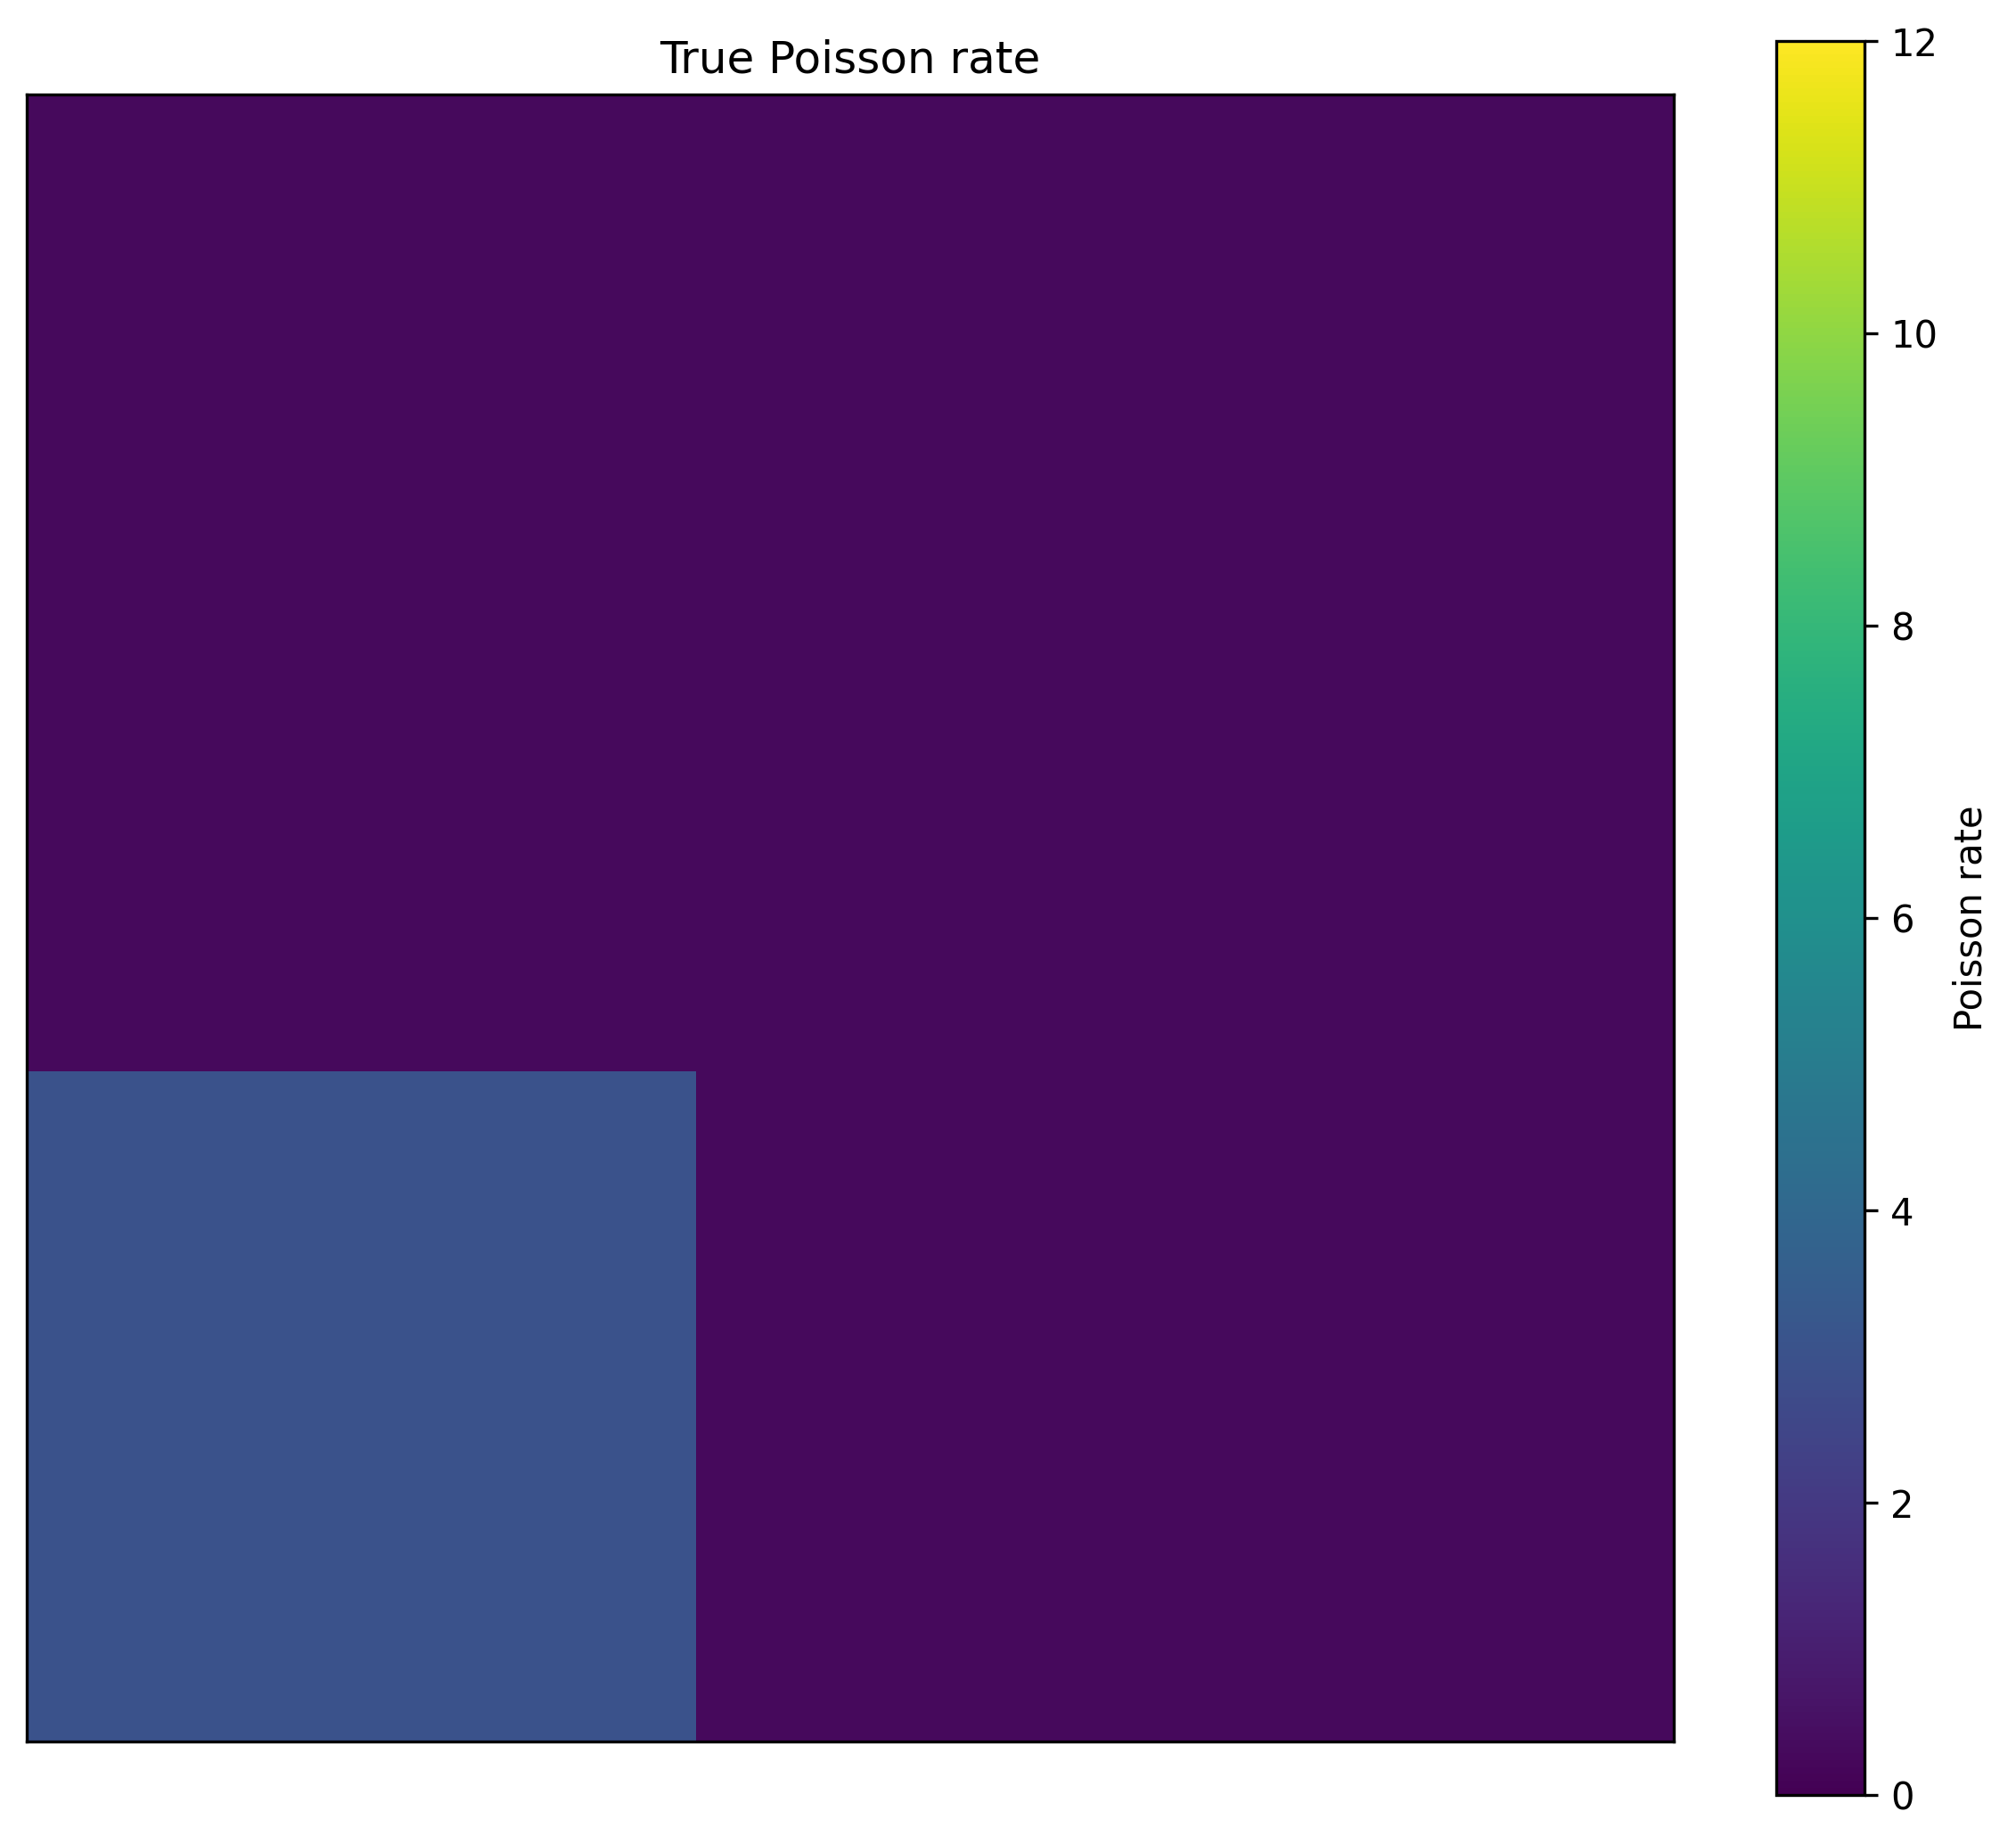
\includegraphics[
    width=\linewidth,
    height=13cm,
    keepaspectratio
]{figures/synthetic_block_true_rate_rho_2_lam_12_var_4.png}

\end{minipage}
\hfill
\begin{minipage}[t]{0.48\linewidth}
\centering

\textbf{Observed counts}

\vspace{0.2cm}

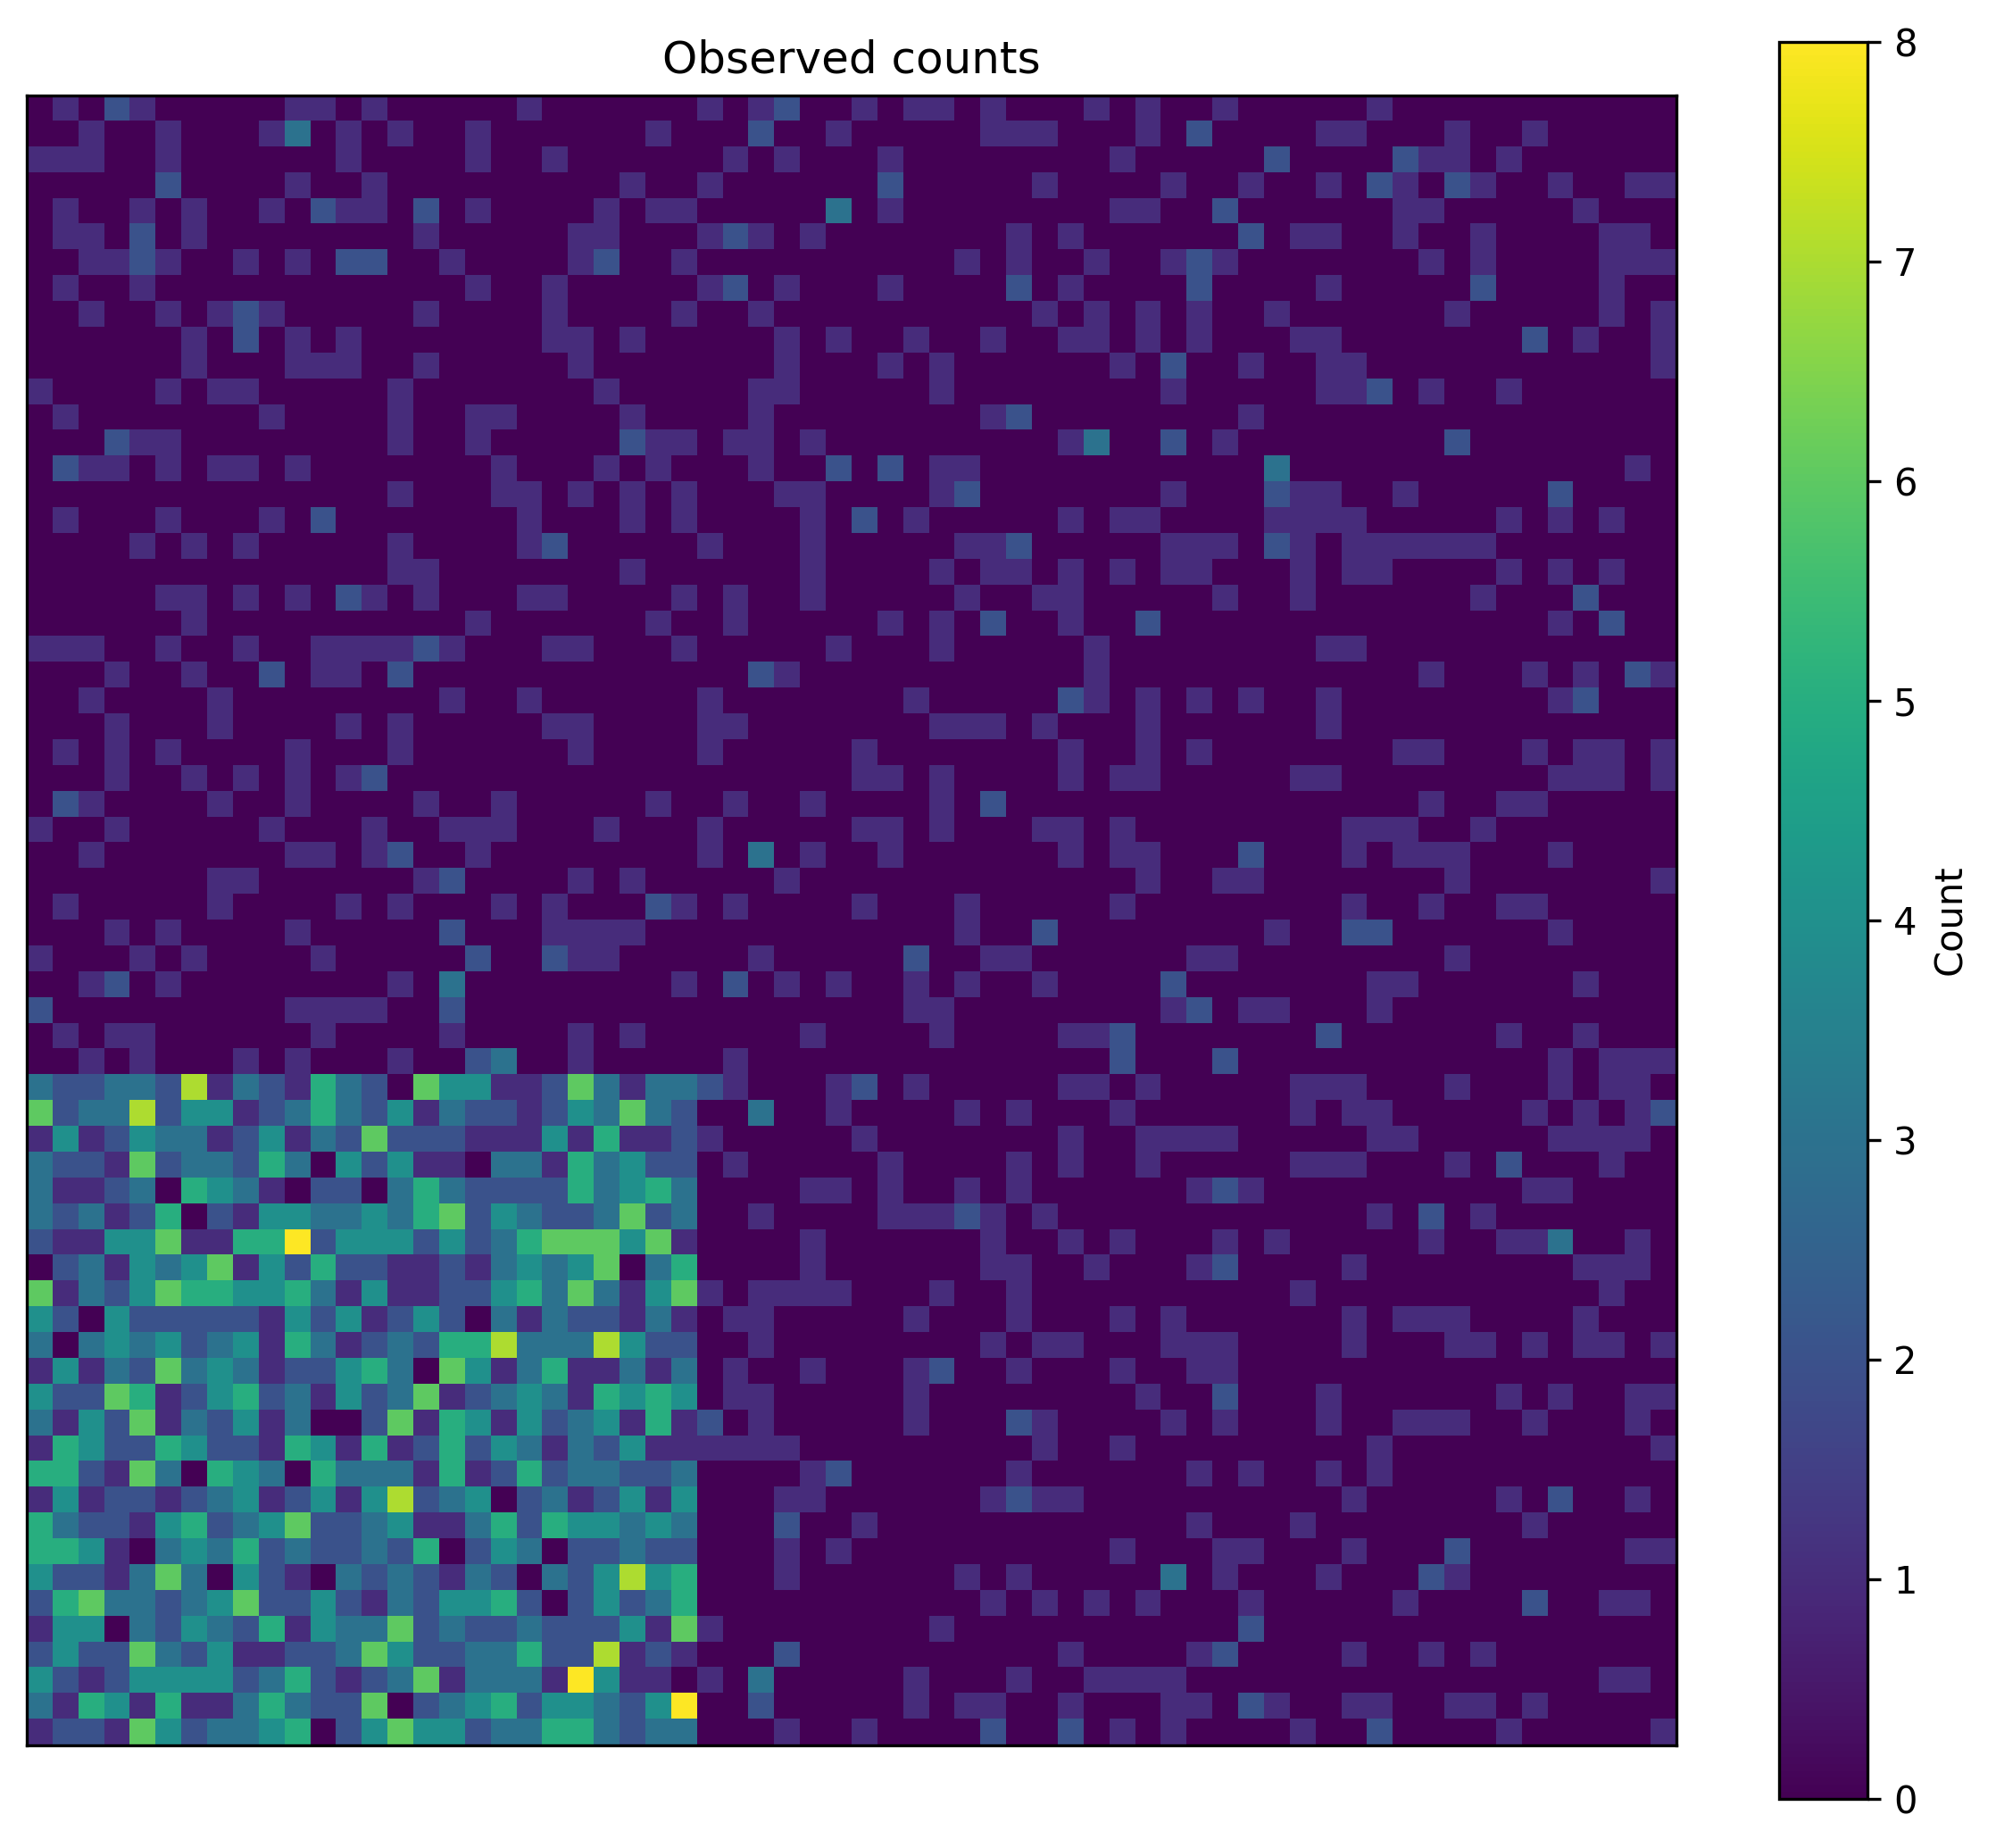
\includegraphics[
    width=\linewidth,
    height=13cm,
    keepaspectratio
]{figures/synthetic_block_observed_counts_rho_2_lam_12_var_4.png}

\end{minipage}

\vspace{0.5cm}

\begin{minipage}[t]{0.48\linewidth}
\centering

\textbf{Posterior mean}

\vspace{0.2cm}

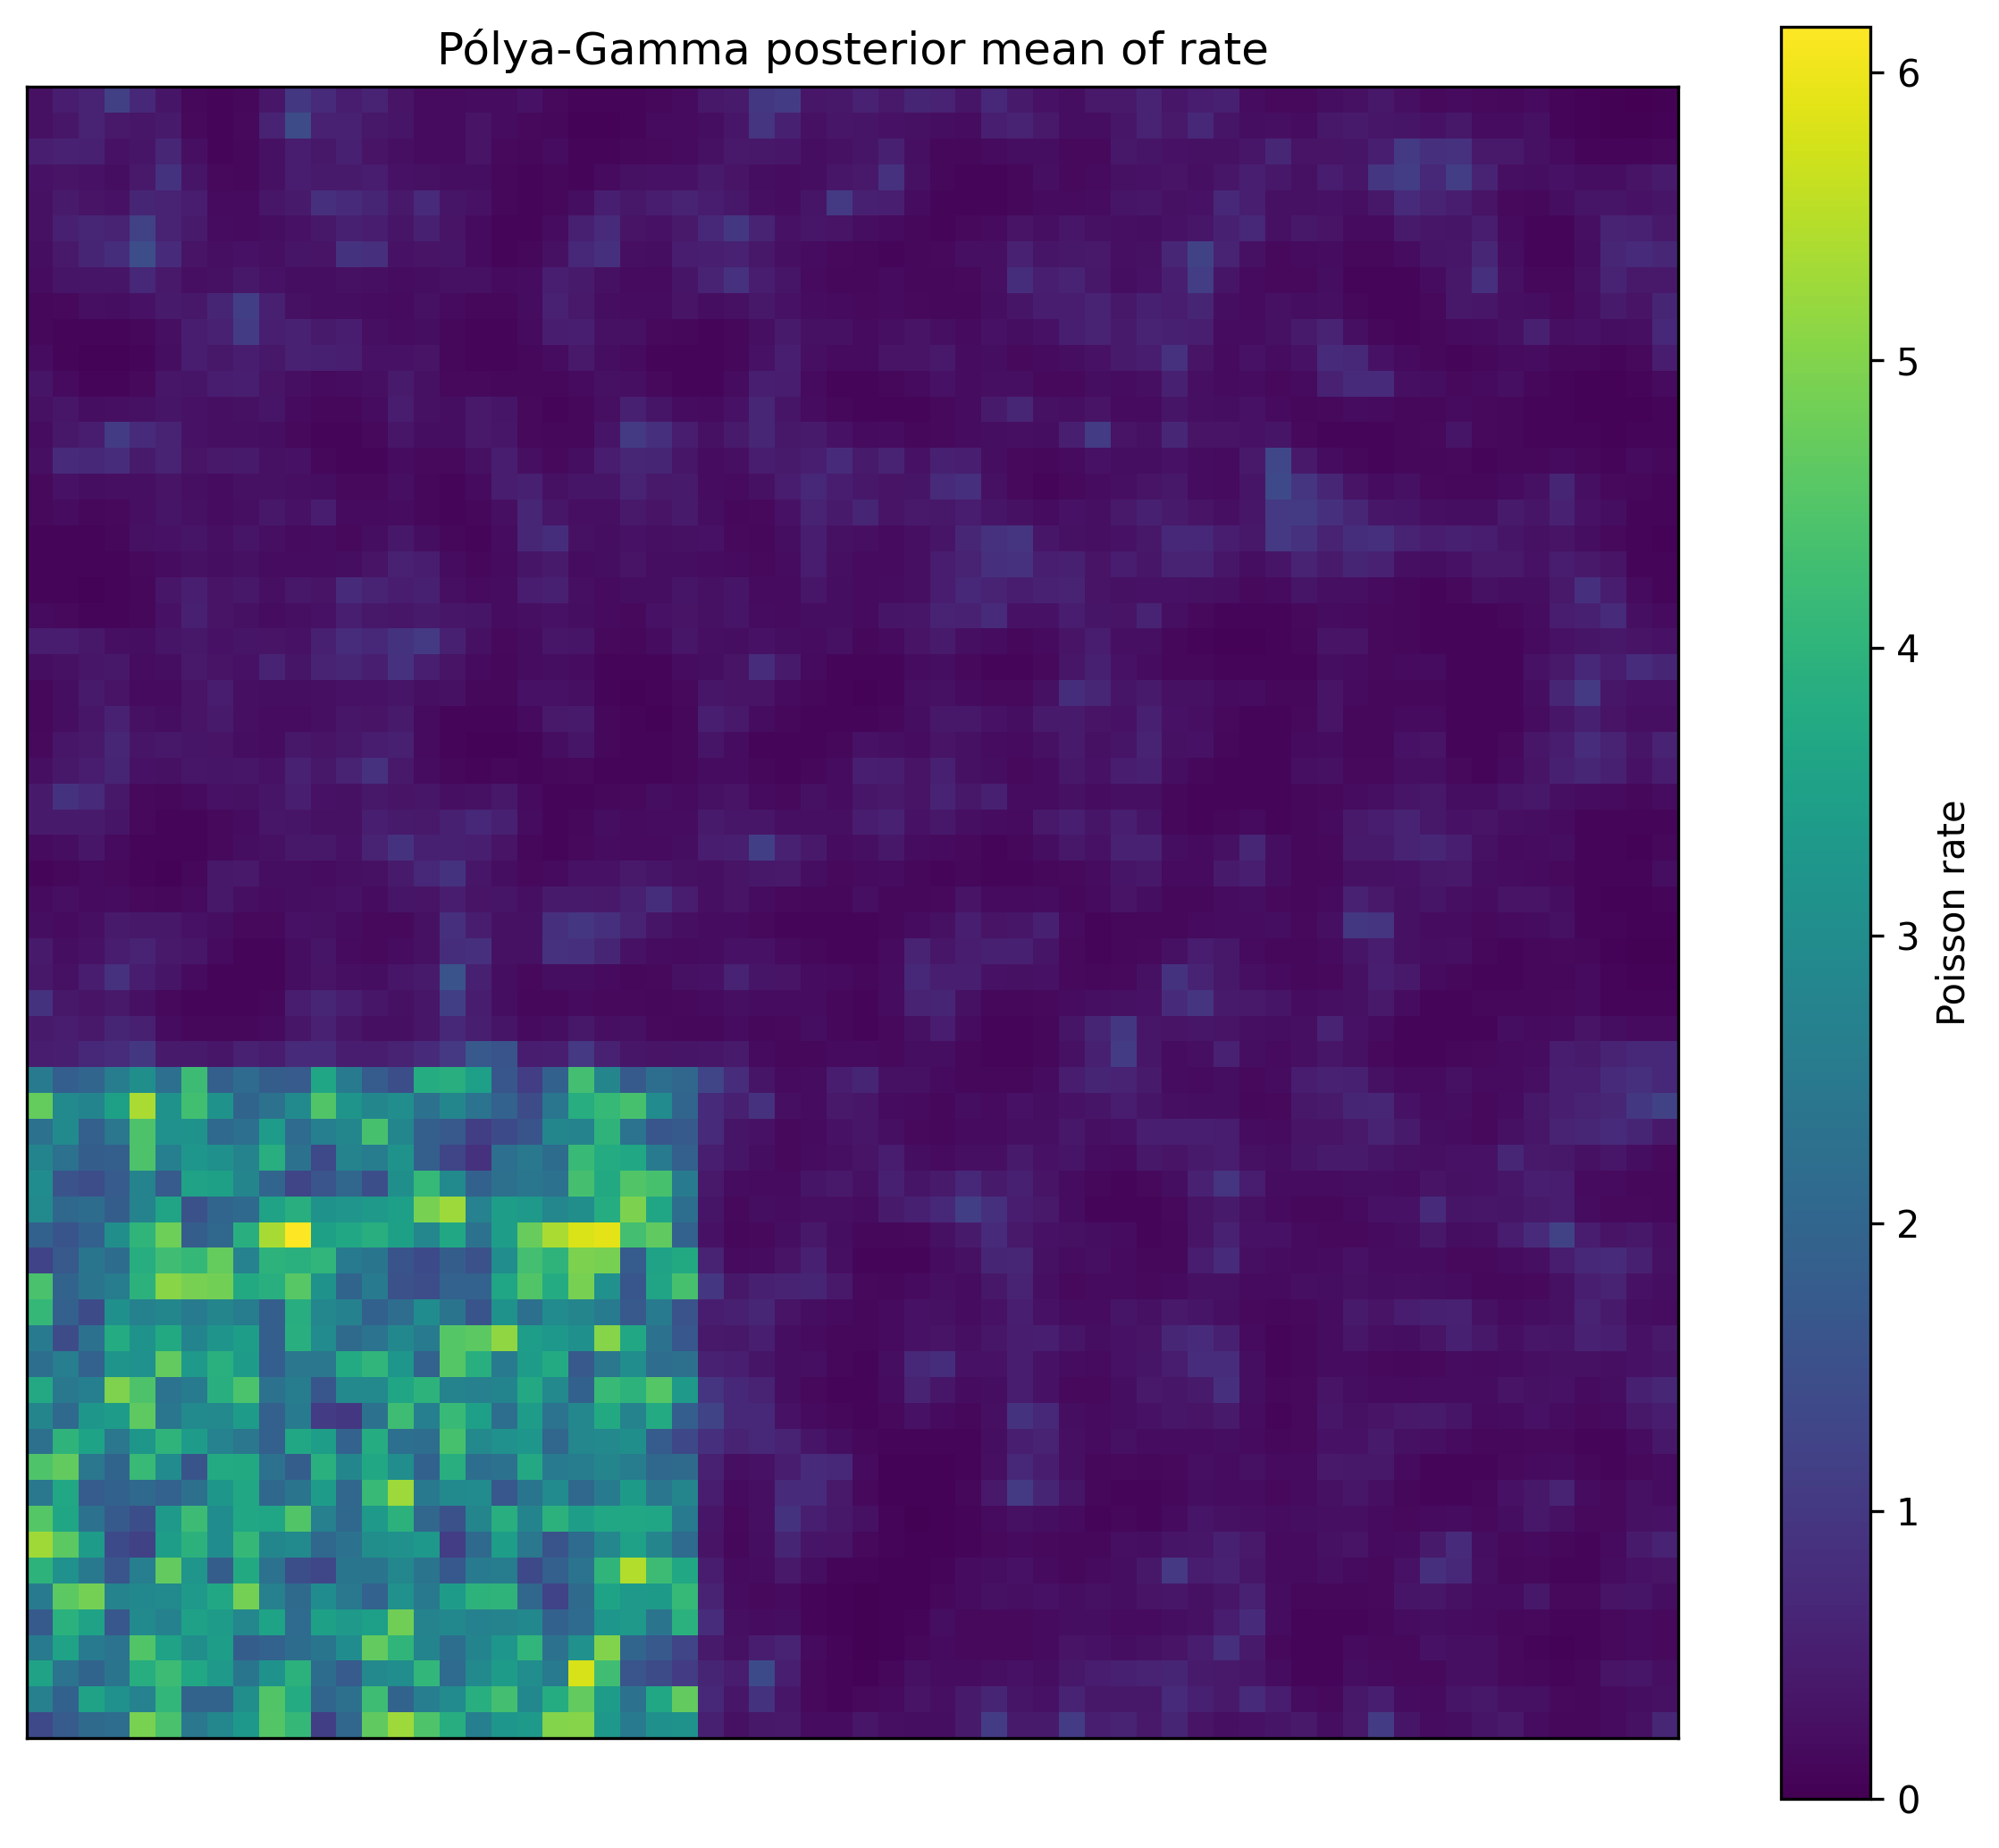
\includegraphics[
    width=\linewidth,
    height=13cm,
    keepaspectratio
]{figures/synthetic_block_posterior_mean_rate_rho_2_lam_12_var_4.png}

\end{minipage}
\hfill
\begin{minipage}[t]{0.48\linewidth}
\centering

\textbf{Posterior mean $-$ truth}

\vspace{0.2cm}

\includegraphics[
    width=\linewidth,
    height=13cm,
    keepaspectratio
]{figures/synthetic_block_posterior_mean_minus_truth_rho_2_lam_12_var_4.png}

\end{minipage}

\vspace{0.4cm}

\textbf{Result.}
The compact high-rate region is recovered, while the sharp boundary
is smoothed by the spatial prior.

\end{block}


% ------------------------------------------------------------
\begin{alertblock}

\begin{itemize}
    \item Large-scale spatial structures are recovered from noisy counts.
    \item Posterior sampling exposes uncertainty not visible in a single MAP estimate.
    \item The spatial prior produces the expected smoothing near sharp boundaries.
\end{itemize}

\end{alertblock}

\end{column}


% ============================================================
% ============================================================
% COLUMN 3
% ITALY
% ============================================================
% ============================================================

\begin{column}{0.32\textwidth}

\begin{block}{Declustered Italian earthquake catalogue}

\begin{columns}[T,onlytextwidth]


\begin{column}{0.46\textwidth}
\vspace{0.5cm}
\centering

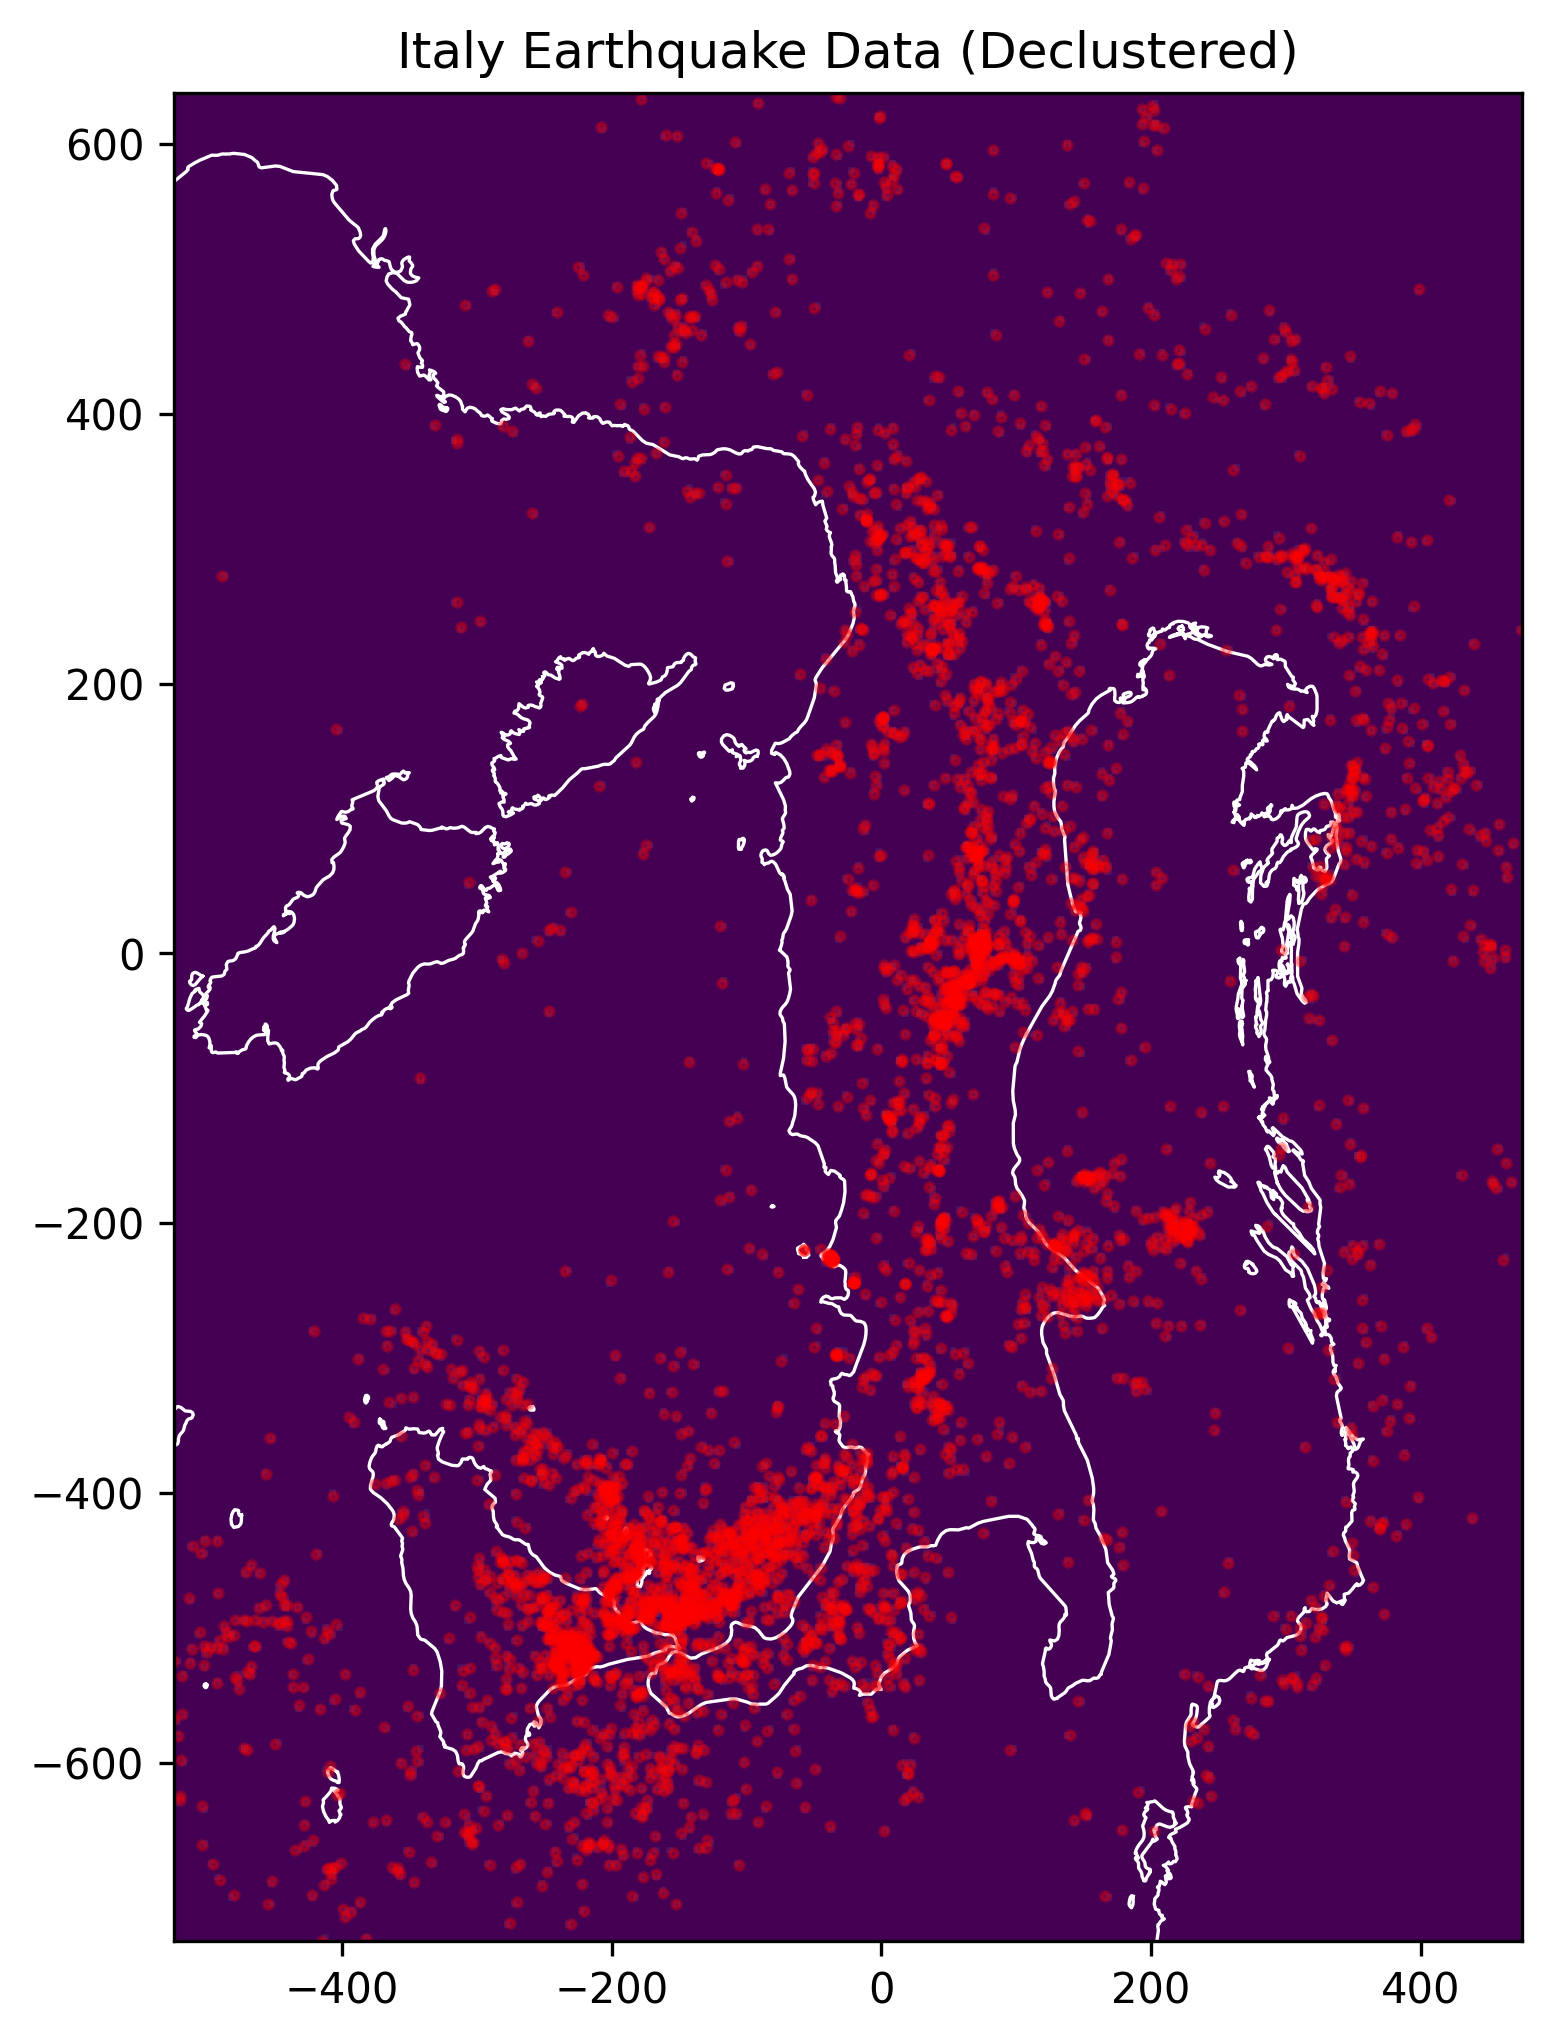
\includegraphics[
    width=\linewidth,
    height=14cm,
    keepaspectratio
]{figures/italy_italy_earthquake_data_bin_5km_declustered.png}

\end{column}


\begin{column}{0.52\textwidth}
\vspace{2cm}
\centering

\small

\begin{tabular}{@{}lrr@{}}
\toprule
Statistic & Original & NND \\
          & catalogue & declustered \\
\midrule
Events          & 11,327 & 4,943 \\
Occupied cells  & 3,518  & 3,230 \\
Cells $\geq 10$ & 135    & 16 \\
Cells $\geq 15$ & 89     & 5 \\
Maximum count   & 279    & 23 \\
Variance / mean & 49.26  & 2.66 \\
\bottomrule
\end{tabular}

\vspace{0.8cm}

\raggedright
\small
NND declustering strongly reduces highly populated cells while
preserving much of the spatial footprint of the catalogue.

\end{column}

\end{columns}

\end{block}



% ------------------------------------------------------------
\begin{block}{Posterior inference}

\begin{minipage}[t]{0.48\linewidth}
\centering

\textbf{Posterior mean}

\vspace{0.2cm}


\includegraphics[
    width=\linewidth,
    height=13cm,
    keepaspectratio
]{figures/italy_posterior_mean_f_bin_5km_declustered.png}

\end{minipage} \hfill%
\begin{minipage}[t]{0.48\linewidth}
\centering


\textbf{Posterior sd of $f$}

\vspace{0.2cm}


\includegraphics[
    width=\linewidth,
    height=13cm,
    keepaspectratio
]{figures/italy_posterior_sd_f_bin_5km_declustered.png}

\end{minipage}

\end{block}


% ------------------------------------------------------------
\begin{block}{MAP versus full posterior}

\centering


\includegraphics[
    width=0.72\linewidth,
    height=13cm,
    keepaspectratio
]{figures/italy_difference_f_bin_5km_declustered.png}

\vspace{0.2cm}

\raggedright

The MAP and posterior mean reproduce similar broad-scale structures,
but posterior sampling additionally provides spatial uncertainty and
reveals where the posterior is asymmetric.

\end{block}


% ------------------------------------------------------------
\begin{block}{Conclusions}


\begin{itemize}
    \item Exact data augmentation gives tractable Gaussian updates.
    \item Synthetic experiments recover the main spatial structures.
    \item The Italy posterior exhibits coherent spatial seismicity patterns.
    \item Posterior sampling provides uncertainty that MAP estimation alone cannot provide.
\end{itemize}

\end{block}

% ------------------------------------------------------------
\begin{block}{References}

\footnotesize

Choi, H. M. \& Hobert, J. P. (2013).
\textit{The Pólya--Gamma Gibbs sampler for Bayesian logistic regression
is uniformly ergodic}.
Electronic Journal of Statistics.

\vspace{0.15cm}

Polson, N. G., Scott, J. G. \& Windle, J. (2013).
\textit{Bayesian inference for logistic models using Pólya--Gamma latent variables}.

\vspace{0.15cm}

Zaliapin, I. \& Ben-Zion, Y.
Nearest-neighbor methods for earthquake clustering and declustering.

\end{block}

\end{column}

\end{columns}

\end{frame}

\end{document}